% !TEX root =  main.tex

\section{Bayesian Experimental Design}
\label{sec:exp-design}

Bayesian experimental design provides a framework for designing experiments in a manner that is optimal from
an information-theoretic viewpoint \citep{chaloner1995bayesian,sebastiani2000maximum}.  By minimizing the entropy in the posterior distribution of the 
parameters of interest, one can maximize the information gathered by the experiment.

Let the parameters of interest be denoted by $\theta \in \Theta$ for which we define a prior distribution $p(\theta)$.
Let the probability of achieving outcome $y\in\mathcal{Y}$, given parameters $\theta$ 
and a design $d \in \mathcal{D}$, be defined by likelihood model $p(y | \theta, d)$.
Under our model, the outcome of the experiment given a chosen $d$ is distributed according to
\begin{equation}
\label{eq:marginal_def}
p(y | d) = \int_{\Theta} p(y,\theta | d) d\theta = \int_{\Theta} p(y | \theta, d) p(\theta) d\theta.
\end{equation}
where we have used the fact that $p(\theta)=p(\theta|d)$ because $\theta$ is independent of the design.
Our aim is to choose the optimal design $d$ under some criterion. 
We, therefore, define a utility function, $U(y,d)$, representing the utility of choosing a design $d$ 
and getting a response $y$.
Typically our aim is to maximize information gathered from the experiment, and so we set 
$U(y,d)$ to be the gain in Shannon information between the prior and the posterior:
\begin{align}
\label{eq:shannon_inf}
U(y,d) &= \int_{\Theta} p(\theta |y, d) \log(p(\theta |y, d)) d\theta -\int_{\Theta} p(\theta) \log(p(\theta))d\theta
\end{align}
However, we are still uncertain about the outcome. Thus, we use the expectation of $U(y,d)$ with respect to $p(y | d)$
as our target:
\begin{align}
\bar{U}(d) & = \int_{\mathcal{Y}} U(y,d) p(y|d) dy\nonumber\\
&=\int_{\mathcal{Y}}\int_{\Theta} p(y,\theta | d)\log(p(\theta |y, d)) d\theta dy - \int_{\Theta} p(\theta) \log(p(\theta)) d\theta \nonumber\\
&=\int_{\mathcal{Y}}\int_{\Theta} p(y,\theta | d)\log\left(\frac{p(\theta |y, d)}{p(\theta)}\right)d\theta dy. 
\label{eq:u_bar_1}
\end{align}
noting that this corresponds to the mutual information between the parameters $\theta$ and
the observations $y$.  The Bayesian-optimal design is then given by
\begin{equation}
\label{eq:d_star}
d^* = \argmax_{d \in \mathcal{D}} \bar{U}(d).
\end{equation}

Finding $d^*$ is challenging because the posterior $p(\theta |y, d)$ is rarely known in closed form.  
To solve the problem, we proceed by rearranging~\eqref{eq:u_bar_1} using Bayes' rule (remembering that
$p(\theta)=p(\theta|d)$):
\begin{align}
\label{eq:u_bar_2}
\begin{split}
\bar{U}(d) = & \int_{\mathcal{Y}}\int_{\Theta} p(y,\theta | d) \log\left(\frac{p(\theta | y, d)}{p(\theta)}\right) d\theta dy \\
=& \int_{\mathcal{Y}}\int_{\Theta} p(y,\theta | d) \log\left(\frac{p(y | \theta, d)}{p(y |d)}\right) d\theta dy \\
=&\int_{\mathcal{Y}}\int_{\Theta} p(y,\theta | d) \log(p(y | \theta, d)) d\theta dy - \int_{\mathcal{Y}} p(y | d) \log(p(y | d))dy.
\end{split}
\end{align}
The first of these terms can now be evaluated using standard MC approaches as the integrand is analytic.  
In contrast, the second term is not directly amenable to standard MC estimation
as the marginal $p(y|d)$ represents an expectation
and taking its logarithm represents a nonlinear functional mapping.  

To derive an estimator, we will now consider these terms separately.  Starting
with the first term,
\begin{align}
\bar{U}_1(d) = &\int_{\mathcal{Y}}\int_{\Theta} p(y,\theta | d) \log(p(y | \theta, d)) d\theta dy
\approx \frac{1}{N} \sum_{n=1}^{N} \log(p(y_n | \theta_n, d)) \label{eq:U1_MC}
\end{align}
where $\theta_n \sim p(\theta)$ and $y_n \sim p(y|\theta=\theta_n, d)$.  We
note that evaluating~\eqref{eq:U1_MC} involves both
sampling from $p(y | \theta, d)$ and directly evaluating it point-wise.
The latter of these cannot be avoided, but in the scenario where we
do not have direct access to a sampler for $p(y | \theta, d)$, we can
use the standard importance sampling trick, sampling instead
$y_n \sim q(y|\theta=\theta_n, d)$ and weighting the samples in~\eqref{eq:U1_MC}
by $w_n = \frac{p(y_n|\theta_n, d)}{q(y_n|\theta_n, d)}$.

Now considering the second term we have
\begin{align}
\bar{U}_2(d) = &\int_{\mathcal{Y}} p(y | d) \log(p(y | d))dy
\approx \frac{1}{N} \sum_{n=1}^{N} \log \left(\frac{1}{M} \sum_{m=1}^{M} p(y_n | \theta_{n,m}, d)\right) \label{eq:U2_MC}
\end{align}
where $\theta_{n,m} \sim p(\theta)$ and $y_n \sim p(y | d)$.  Here we can sample the latter by first sampling an otherwise unused $\theta_{n,0} \sim p(\theta)$ and 
then sampling $y_n \sim p(y | \theta_{n,0}, d)$.  Again we can use importance sampling if 
we do not have direct access to a sampler for $p(y | \theta_{n,0}, d)$.

Putting~\eqref{eq:U1_MC} and~\eqref{eq:U2_MC} together (and renaming
$\theta_n$ from~\eqref{eq:U1_MC} as $\theta_{n,0}$ for notational
consistency with ~\eqref{eq:U2_MC})  we now have the following complete estimator
given in the main paper and implicitly used by \cite{myung2013tutorial} 
and \cite{ouyang2016practical} amongst others
\begin{align}
\label{eq:exp-des-nmc}
\bar{U}(d) 
& \approx  
\frac{1}{N} \sum_{n=1}^{N} \left[ \log(p(y_n | \theta_{n,0},d)) 
- \log \left(\frac{1}{M} \sum_{m=1}^{M}p(y_n | \theta_{n,m},d)\right) \right]
\end{align}
where $\theta_{n,m} \sim p(\theta) \; \forall m \in 0:M, \;n \in 1:N$ and $y_n \sim p(y|\theta=\theta_{n,0}, d) \; \forall n \in 1:N$.

We now show that if $y$ can only take on one of $C$ possible values ($y_1, \ldots, y_C$), 
we can achieve significant improvements in the convergence rate by using a similar to that
introduced in Section 3.2 to convert to single MC estimator:
\begin{align}
\bar{U}(d)=&\int_{\mathcal{Y}}\int_{\Theta} p(y,\theta | d) \log(p(y | \theta, d)) d\theta dy - \int_{\mathcal{Y}} p(y | d) \log(p(y | d))dy \nonumber\\
=& \int_{\Theta} \left[\sum_{c=1}^{C} p(\theta) p(y_c|\theta, d) \log(p(y_c | \theta, d)) \right] d\theta
-\sum_{c=1}^{C} p(y_c | d)\log(p(y_c | d)) \nonumber \\
\begin{split}
\approx& \label{eq:u_bar_MC}
\frac{1}{N} \sum_{n=1}^{N} \sum_{c=1}^{C} p(y_c | \theta_n, d) \log\left(p(y_c | \theta_n, d)\right) \\
&- \sum_{c=1}^{C} \left[\left(\frac{1}{N}\sum_{n=1}^{N} p(y_c | \theta_n, d)\right) \log \left(\frac{1}{N} \sum_{n=1}^{N} p(y_c | \theta_n, d)\right) \right]
\end{split}
\end{align}
where $\theta_n \sim p(\theta) \quad \forall n \in 1,\dots,N$.  As $C$ is a fixed constant,
the MSE for first term clearly converges at the standard MC error rate of $O(1/N)$.  Similarly each
$\hat{P}_N(y_c | d) = \frac{1}{N}\sum_{n=1}^{N} p(y_c | \theta_n, d)$ term also converges at a rate 
$O(1/N)$ to $p(y_c | d)$.  Now noting that $\hat{P}_N(y_c | d) \le 1$ and that $f(x) = x \log x$ is Lipschitz
continuous in the range $(0,1]$, each $\hat{P}_N(y_c | d) \log \left(\hat{P}_N(y_c | d)\right)$ 
term must also converge at the MC error rate if $p(y_c | d)>0 \; \forall c=1,\dots,C$.  
Finally if we assume that when $p(y_c | d)=0$ then $\hat{P}_N(y_c | d)=0$
almost surely for sufficiently large $N$, then the second term also converges at the MC error when
$p(y_c | d)=0$.  We now have a finite sum of terms which each convergence to $\bar{U}(d)$ with MC
MSE rate $O(1/N)$, and so the overall estimator~\eqref{eq:u_bar_MC} must also converge at this rate.
This compares to $O(1/T^{2/3})$ for~\eqref{eq:exp-des-nmc} (assuming we take $N \propto M^2$), noting that generating $T$ samples for~\eqref{eq:exp-des-nmc} has the same cost up to a constant factor as generating $N$ for~\eqref{eq:u_bar_MC}.
To the best of our knowledge, this is the first introduction of this superior estimator in the literature.

We finish by showing that the theoretical advantages of this reformulation also leads to empirical gains in the estimation of $\bar{U}(d)$.  For this, we consider a model used in psychology experiments for delay discounting introduced by \cite{vincent2016hierarchical}.  Our experiment comprises of asking questions of the form \emph{``Would you prefer $\pounds A$ now, or $\pounds B$ in $D$ days?''} and we wish to choose the question  variables $d = \{A,B,D\}$ in the manner that will give the most incisive questions.  The target participant is presumed to have parameters $\theta=\{k,\alpha\}$ and the following response model
\begin{equation}
y \sim \mathrm{Bernoulli} \left(0.01 + 0.98 \cdot \Phi\left(\frac{1}{\alpha} \left(\frac{B}{1+e^k D}-A\right)\right)\right)
\end{equation}
where $y=1$ indicates choosing the delayed response and $\Phi$ represents the cumulative normal distribution.  As more questions are asked, the distribution over the parameters $\theta$ is updated, such
that the most optimal question to ask at a particular time depends on the previous questions
and responses.  For the sake of brevity, when comparing the performance of~\eqref{eq:exp-des-nmc} and~\eqref{eq:u_bar_MC} we will neglect the problem of how best to optimize the design, and consider
only the problem of evaluating $\bar{U}(d)$.  We will further consider the case where $B=100$ and $D = 50$ are fixed and we are only choosing the delayed value $A$.
We presume the following distribution on the parameters
\begin{align*}
k &\sim \mathcal{N}(-4.5,0.5^2) \\
\alpha &\sim \Gamma(2,2).
\end{align*}
We first consider convergence in the estimate of $\bar{U}(d)$ for the case $A=70$ for our suggested method~\eqref{eq:u_bar_MC} and the na\"{i}ve solution~\eqref{eq:exp-des-nmc}, the results of which are shown in Figure~2a in the main paper. 
Here we see that the convergence rates of the two methods are both as expected and that our suggested method offers significant empirical performance improvements.  

\begin{figure}[t]
		\centering
		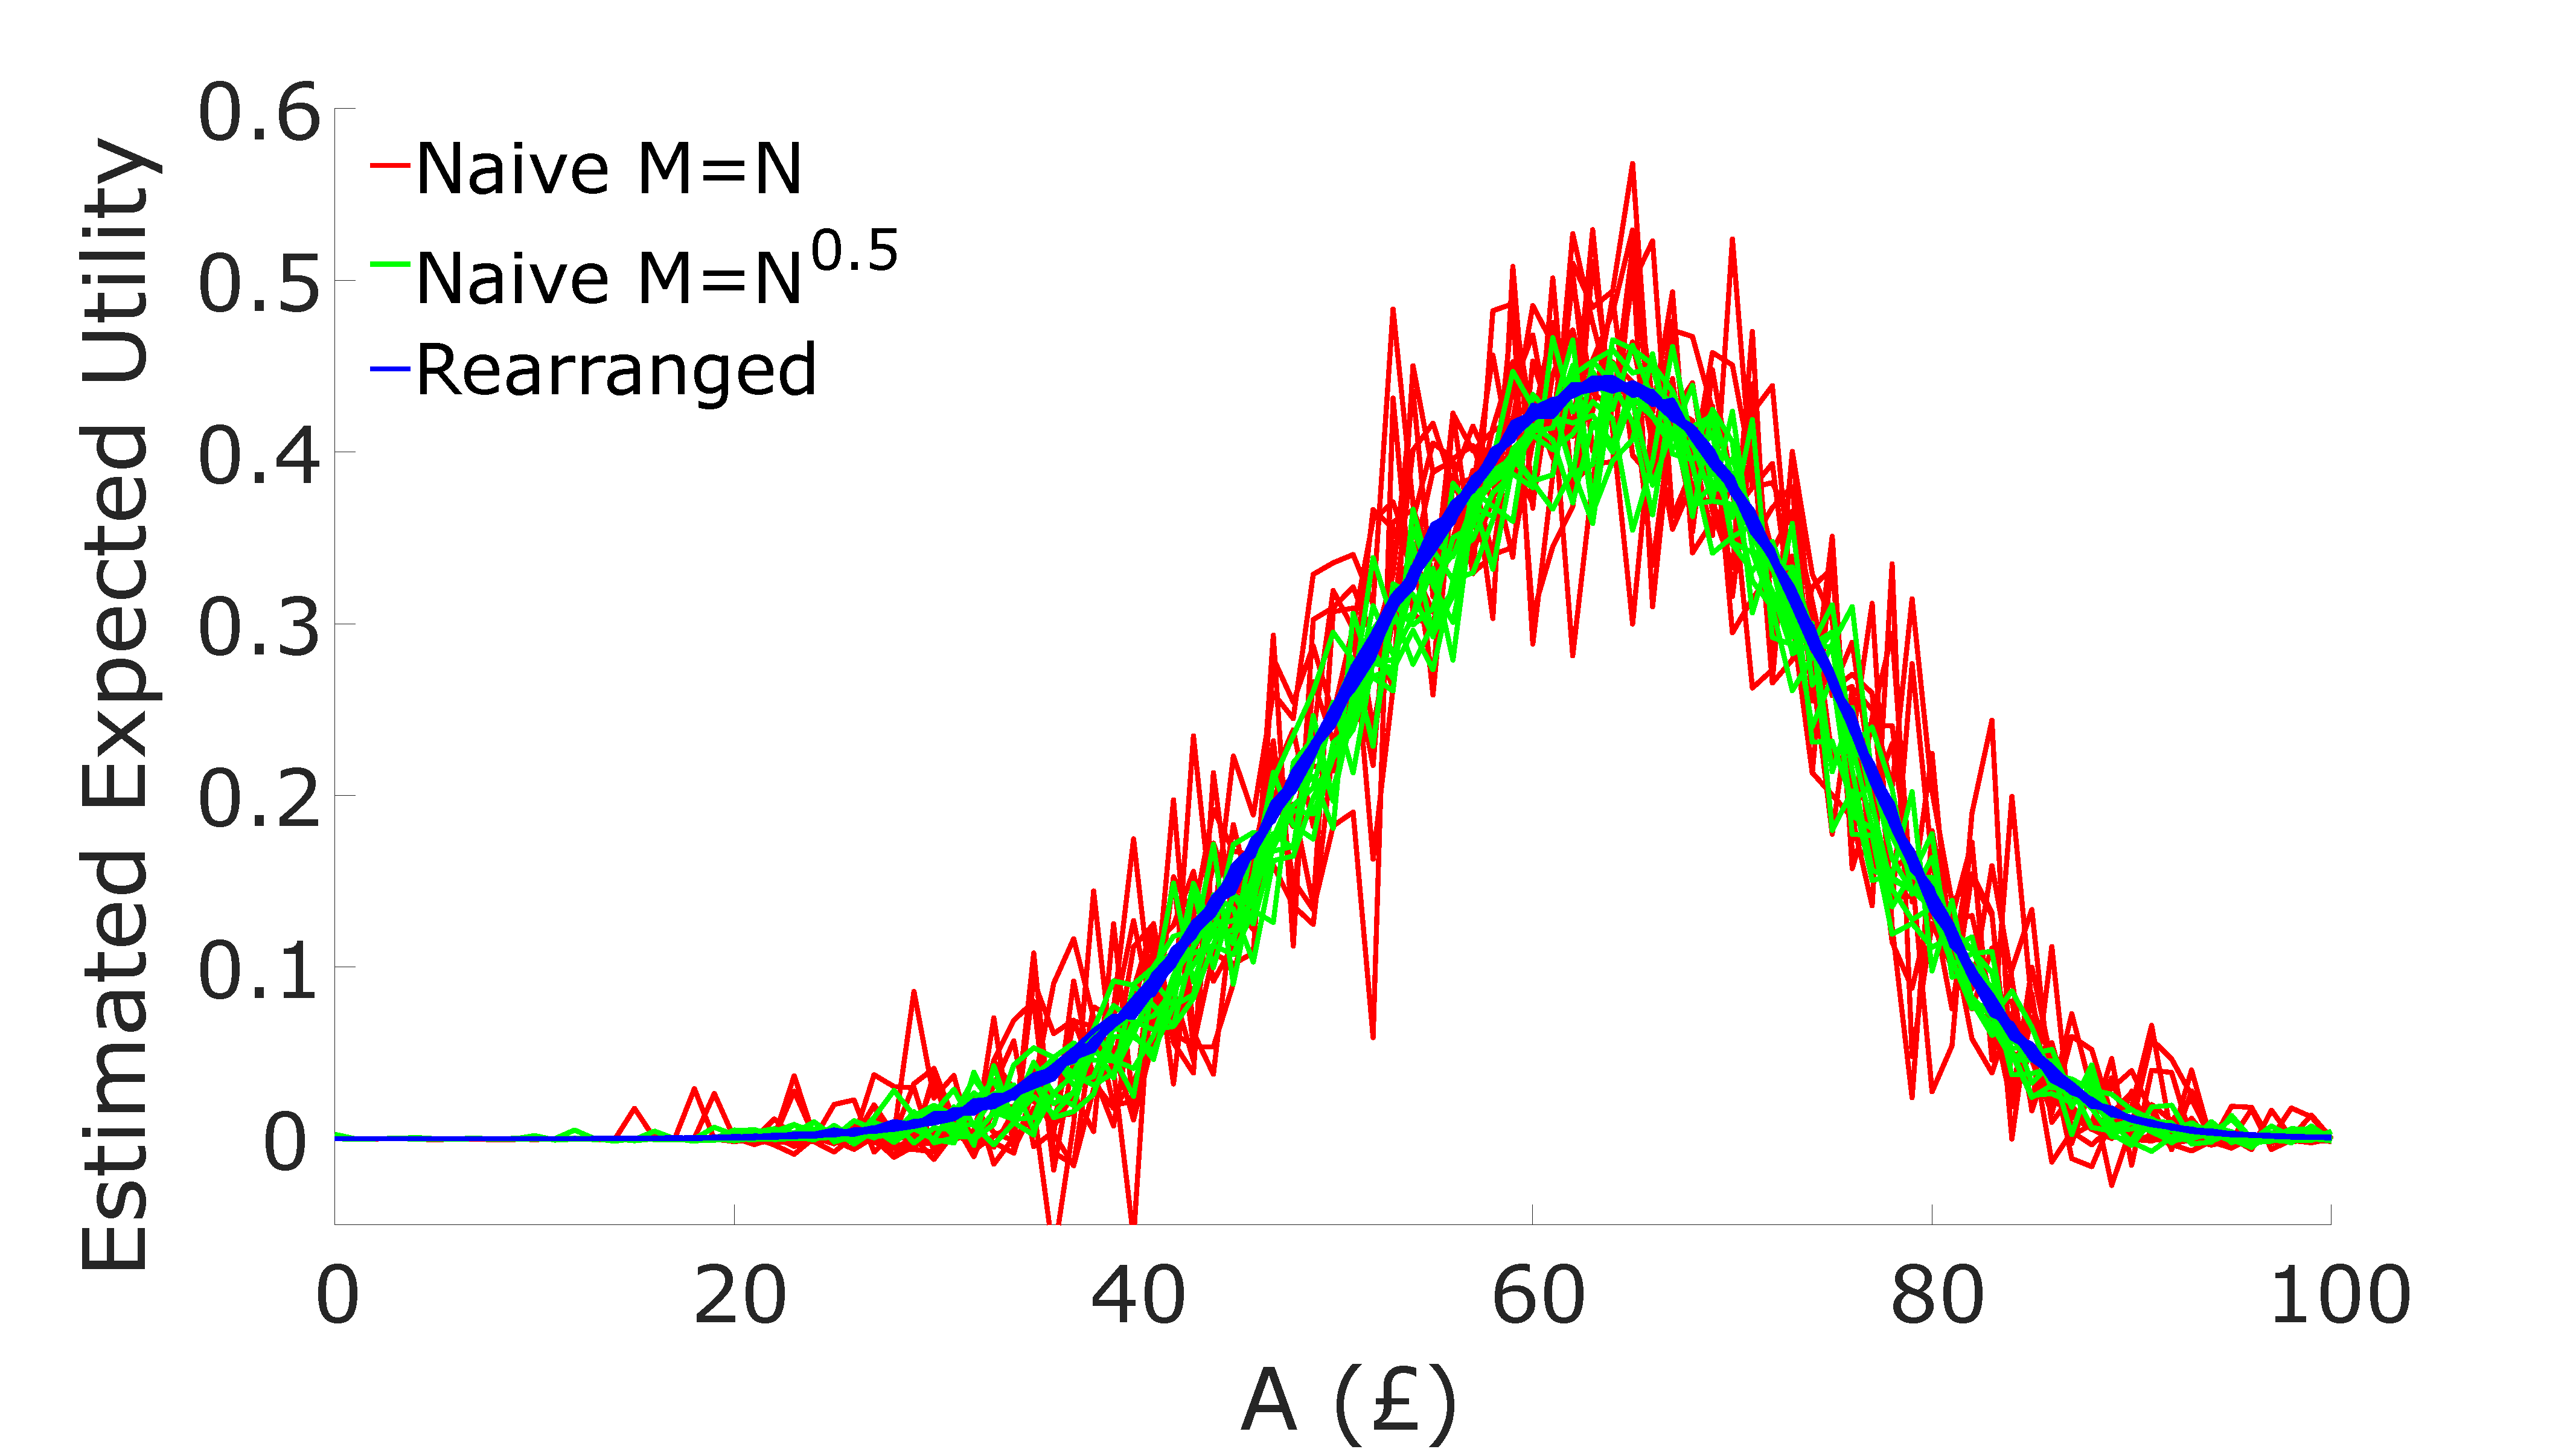
\includegraphics[width=0.49\textwidth,trim={1.5cm 0 3.5cm 0},clip]{dscan_2}
		\caption{Estimated expected utilities $\bar{U}(d)$for 
		different values of one of the design parameters $A \in \{1,2,\dots,100\}$ given a fixed total
		sample budget of $T=10^4$.  Here the lines correspond to 10 independent runs, showing
		that the variance of \eqref{eq:exp-des-nmc} is far higher than \eqref{eq:u_bar_MC}.\label{fig:exp-d-scan}}
\end{figure}


We next consider setting a total sample budget $T=10^4$ and look at the variation in the estimated values of $\bar{U}(d)$ for different values of $A$ for the two methods as shown in Figure~\ref{fig:exp-d-scan}.
This shows that the improvement in MSE leads to clearly visible improvements in the characterization of $\bar{U}(d)$ that
will translate to improvements in seeking the optimum.
